\documentclass[11pt]{report}
\usepackage[utf8]{inputenc}

\usepackage[backend=bibtex]{biblatex}
\addbibresource{references.bib}
\usepackage{multirow}
\usepackage{graphicx}
\graphicspath{ {images/} }
\usepackage[compact]{titlesec}
\usepackage{enumitem}

\usepackage{etoolbox}
\makeatletter
\patchcmd{\chapter}{\if@openright\cleardoublepage\else\clearpage\fi}{}{}{}
\makeatother

\usepackage{tocloft}
\setlength{\cftbeforetoctitleskip}{0pt}

\usepackage{listings}
\usepackage{color}

\definecolor{dkgreen}{rgb}{0,0.6,0}
\definecolor{gray}{rgb}{0.5,0.5,0.5}
\definecolor{mauve}{rgb}{0.58,0,0.82}

\lstset{frame=tb,
	language=Java,
	aboveskip=3mm,
	belowskip=3mm,
	showstringspaces=false,
	columns=flexible,
	basicstyle={\small\ttfamily},
	numbers=none,
	numberstyle=\tiny\color{gray},
	keywordstyle=\color{blue},
	commentstyle=\color{dkgreen},
	stringstyle=\color{mauve},
	breaklines=true,
	breakatwhitespace=true,
	tabsize=3
}

\title{
	{Exploring the Applications of Dynamic Programming}
}
\author{Bradley Hunt}
\date{May 2017}

\begin{document}

\maketitle

\tableofcontents
\newpage
\chapter{Introduction}
\section{Motivation}

% Initial Intro
One of the key features in the field of computer science is the constant strive for improvement. Whether it be a piece of hardware, software or an algorithm, it is ideal to continually search for new ways to improve on a variety of aspects such as usability, structuring and, perhaps most importantly; performance. Dynamic programming is a method that captures this constant push for faster, more efficient problem solving. As a model of programming, it holds the core purpose of breaking existing recursive problems down into smaller subproblems to allow for greater efficiency in the solving process as well as in general optimization.
\smallbreak

% What I'm doing with the project - Core of the diss
This project looks at the dynamic programming method of implementation and how it can be applied to ten computational problems to improve upon their base method and increase the efficiency of solving. From this a clear understanding can be obtained of the advantageous elements of implementing a dynamic programming approach to improve upon existing solutions to problems. For each problem the premise and strategy for solving will be explored through documentation. This documentation introduces the premise of the problem in detail as well as providing written examples to demonstrate this in a clear, understandable form. Following this, the approach to writing an algorithm to solve the problem is discussed and demonstrated in a fashion meant to be easily understood by somebody with limited dynamic programming knowledge, while also retaining usefulness for those who are knowledgeable in that field. Additionally the real world applications of these problems will be explored, in order show just how wide the usage of dynamic programming techniques can be spread. 
\smallbreak

% Java programs intro
Alongside this , each problem tackled in this project has an accompanying Java program which exhibits the dynamic programming method of solving that particular problem. These are intended to provide greater understanding of the computational process behind each problem and how dynamic programming assists in this way. Each Java program will show how the core dynamic programming principles can be applied to a more specific problem, meaning links between the programs can be highlighted as well as more unique applications of the technique.\\


Below is a full list of the dynamic programming problems that are explored through this project:

\begin{table}[h]
	\resizebox{\textwidth}{!}{%
		\begin{tabular}{ll}
			• Minimum Coin Change Problem & • Longest Palindromic Substring Problem \\
			• Longest Increasing Subsequence Problem & • Maximum Square Sub-Matrix with all 1's Problem \\
			• Longest Common Subsequence Problem & • Subset Sum Problem \\
			• Edit Distance Problem & • Text Justification Problem \\
			• String Interleaving Problem & • Word Break Problem
		\end{tabular}%
	}
\end{table}

% Project Uses & achievements
This project aims to be a concise educational resource for the topic of dynamic programming, mainly covering how it can be implemented in the process of problem solving. If somebody is unaware of dynamic programming and requires an idea of what the concept is and how it can be easily applied to a set of problems, this project will be able to provide assistance and relative guidance in how to approach a dynamic programming solution. The problems explored can also more explicitly provide insight into specific solutions to problems, given that the Java code is referenced as well as their common applications.
\smallbreak

% Achievements 
Through this project I have achieved what I set out to do, which was to satisfyingly document and program ten dynamic programming problems which I personally found to be interesting to research and understand. Adding to this, through the development of Java programs for each problem, further educational merit can be obtained as well as achieving fully-functional implementation of ten interesting algorithm focused pieces of code.
\smallbreak

\par\noindent
% Aims
To summarise, this projects three key aims are to:
\begin{itemize}
	\item Understand the benefits of a dynamic programming approach to algorithmic problem-solving
	\item Document and achieve understanding of ten different dynamic programming problems
	\item Implement each of the ten problems into functioning Java programs
\end{itemize}


\section{Document Outline}


\chapter{Background}
\section{History of Dynamic Programming}
Initially the term \textit{Dynamic Programming} was used by Richard Bellman, a mathematician, in the 1940s to describe the process of solving problems where one needs to find the best decisions one after another. He would later refine his definition in 1953 to refer to nesting smaller decision problems inside of larger problems, which is what remains the modern definition \cite{bellman}. The word \textit{dynamic} was chosen by Bellman due to the time-varying aspect of the problems and because it sounded impressive \cite{dynamic}. \textit{Programming} was chosen as to refer to the use of the method to find an optimal program and as a synonym to the word planning. Upon establishment of this topic, dynamic programming began to grow and became recognized as a substantial area of interest within the field of computer science. As the field of Computer Science expanded over the years, dynamic programming remains a relevant topic with a multitude of algorithms making use of the method.

\section{Dynamic Programming Overview}
Dynamic programming is both a mathematical optimization method and a computer programming method. In both contexts it refers to simplifying a complicated problem by breaking it down into simpler subproblems in a recursive manner. These subproblems are each solved just once and their solutions are stored - ideally, using a memory-based data structure. The next time the same subproblem occurs, instead of recomputing its solution, the previously computed solution is looked up, thus saving computation time at the expense of some expenditure in storage space\cite{dynamic-wiki}. Dynamic programming is applicable to problems exhibiting two specific properties: optimal substructure and overlapping subproblems.
\smallbreak
A problem is said to have optimal substructure if an optimal solution can be constructed efficiently from optimal solutions of its subproblems\cite{design-manual}. While a problem is said to have overlapping subproblems if the problem can be broken down into subproblems which are reused several times or a recursive algorithm for the problem solves the same subproblem over and over rather than always generating new subproblems\cite{IntroAlgo}. If a problem has both of these properties then a dynamic programming approach to problem solving is applicable. 

\section{Related Work}
As part of the undertaking of this project, I made sure to research the topic of dynamic programming in relative depth in order to gain a proper understanding of the topic. In searching for books and research papers covering dynamic programming, I identified several which I felt were worthwhile and helpful to use as reference points due to a close relation to the aspects of dynamic programming that I wish to study. Firstly, \textit{Dynamic Programming in Computer Science}\cite{DPiCS} is a 1979 paper written by Kevin Q. Brown which somewhat generally introduces the topic of dynamic programming in a relatively easy to understand fashion. It also provides detailed examples of dynamic programming problems and algorithms and the theory behind them. I found this paper provided me with a good introduction to the topic and it was useful to return to later once I had learned some of the greater context regarding dynamic programming, given the detailed documentation. Even if it displayed the topic more mathematically complex than I wished to go for my project.
\smallbreak

Another paper I red through was \textit{Learning to act using real-time dynamic programming} \cite{learning2act}, written by Andrew G. Barto, Steven J. Bradtke and Satinder P Singh. This paper primarily looks at the use of dynamic programming in artificial intelligence. I found that its coverage of a variety of dynamic programming problems and general theory were useful in understanding the greater application of the dynamic programming method. The paper presents and documents a variety of problems that mainly focus on the learning capabilities through memoization techniques. While my approach to this topic is more general and implementation focused, this paper provided useful information on the topic and was helpful in understanding the variety of applications that dynamic programming allows for. 
\smallbreak

The book \textit{Introduction to Algorithms} by Thomas H. Cormen, Charles E. Leiserson, Ronald L. Rivest and Clifford Stein has a chapter devoted to dynamic programming \cite{IntroAlgo}. Chapter 15 of the book covers four dynamic programming problems at length, including the Longest Common Subsequence problem, which I chose to be one of the first problems to look into and implement myself. This chapter of the book also explores the dynamic programming method with a section focusing in on the two key concepts within the topic. This chapter of the book was very useful for me as a concise introduction to the topic as well as providing some inspiration regarding how I would present my own work and approach the project as a whole.
\smallbreak

Similarly another book, \textit{The Algorithm Design Manual} by Steven S Skiena, has a chapter devoted to dynamic programming \cite{design-manual}. In chapter 8 of the book, a selection of dynamic programming problems are discussed in depth as well as providing code and some diagrams for the various problems. The book also observes links between different problems and how the understanding of one allows for easier understanding of a similar related problem. Similar to \textit{Introduction to Algorithms}, this book was very helpful in providing an idea of how I should present my work and the sorts of research and documentation I'd have to delve into for each dynamic programming problem I would tackle. It also covered certain problems I chose to implement myself, namely the edit distance and longest increasing subsequence problems.
\smallbreak

One last book that I read through to assist in working on this project was \textit{Dynamic Programming For Coding Interviews} which is written by Meenakshi \& Kamal Rawat \cite{interviews}. Unlike the previous books and research papers mentioned, I read this book later in my project development time line, when I had already began properly programming. This book was very helpful in re-enforcing the key concepts of dynamic programming in my mind as well as how to approach the problem solving method. Mostly, this book goes into detail on the method of dynamic programming for problem solving, while also containing a lot of useful examples, including a few problems that I implemented for my project; the minimum coin change and longest palindromic subsequence problems.


\chapter{Project Specification}
\section{Feature Specification}
For this project I initially set out to implement several  different dynamic programming problems into Java programs with helpful output. To begin with I primarily researched into the topic and looked into a variety of problems that I could possibly implement. After making a list of problems I found to be applicable to possibly be covered through this project and producing minimal notation on each of them, I narrowed the list down to ten problems. The initial stages of software design were spent understanding the problems in greater detail and documenting their workings. This then allowed more confidence when it came to actually start properly coding the problems as well as saving time when it came to writing up about each problem for the implementation section of this dissertation.
\smallbreak
While each of the ten programs have their own set of specifications, the basic shared feature that each of them require was to be able to solve the given problem by taking in appropriate input. For each problem this was achieved by having the program's core dynamic programming algorithm work correctly and to then return either true or false, or the length of the answer according to what data was input for which separate program. Additionally the optional feature I set out for each program to have was expanded output, so instead of returning simply true or false, more useful data could be output. As an example, the first program I implemented was the minimum coin change problem. Initially my main focus was on developing the dynamic programming algorithm and in such once I got that working the output was minimal, simply returning the minimum number of coins required to make change for a given amount. However I then expanded the code and ended up producing better output which also returned the values of each of the minimum number of coins required to make change for a given amount.
\smallbreak
Another key feature was for each of the problems to be commented to a satisfying level. My aim was to provide high quality Java comments which would be able to assist in helping somebody understand the specific dynamic programming problem. As I had researched a lot into how these problems are structured and how to go about the problem-solving process, I made sure to write detailed comments for each program and continually update them as I changed the programs around. I also included Javadoc comments for each class and method to keep the code and comments to a professional standard as well as achieving a higher level of user-friendliness.

\begin{figure}[h]
	\centering
	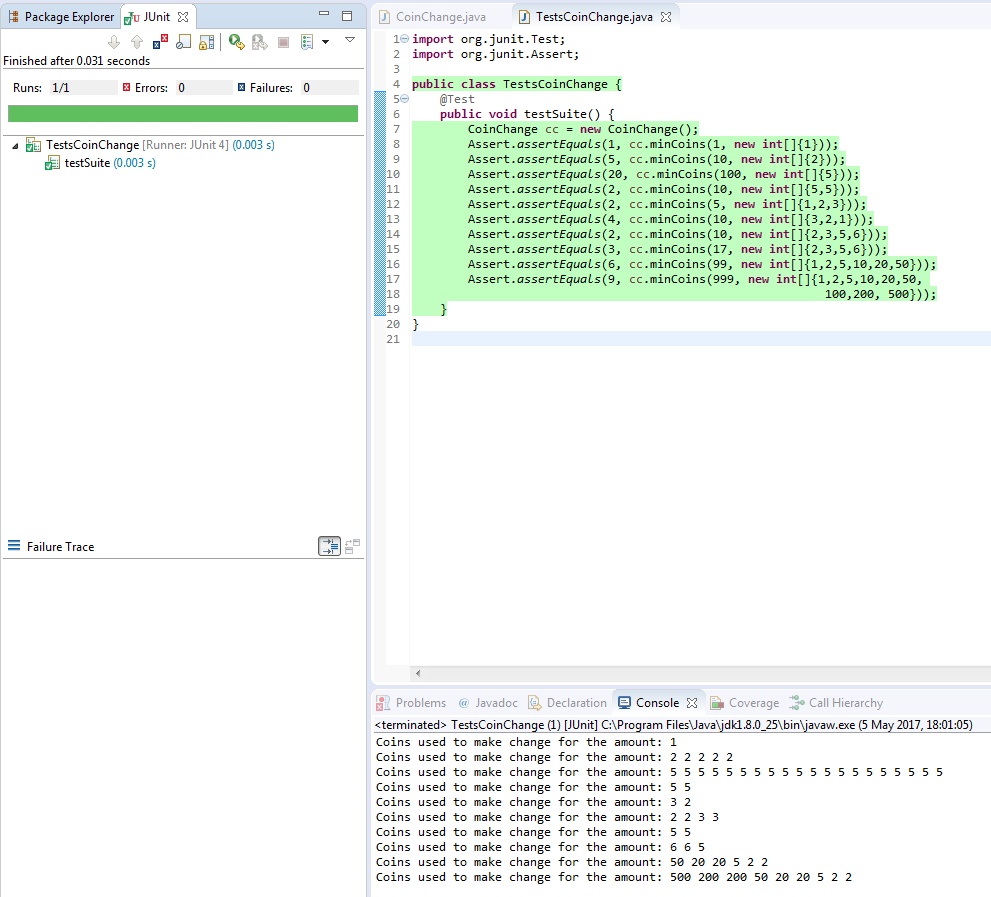
\includegraphics[width=0.8\textwidth]{testing}
	\caption{The test class for minimum coin change problem running Eclemma}
\end{figure}

The final stage of developing the programs was testing. For each program, except for the implementation of the text justification problem, I used EclEmma to perform white-box testing through the Eclipse Java IDE formulated in JUnit. I wrote series of test cases which tested the different sorts of input onto the core methods of each program. Due to the complicated input for the text justification problem, I did testing for that manually myself. The outcome of testing was very positive and by the end of the process I had had concluded that each program was working as intended with no clear errors made in the process. Each test class obtained full coverage over the test cases I created. Through testing I was also able to more clearly evaluate my work, showing the versatility of each problem in terms of input and output.


\section{Technology Choices}
The core technology choice I had to make for this project was with which programming language to write the programs in. I assessed a few different languages to see what advantages they had when it comes to implementation of dynamic programming problems specifically. The biggest advantage any one language that I looked into had was Python, as it allows for memoization to be done automatically, due to functions being first-class objects. This in turn can simplify the implementation of a dynamic programming problem by a fair margin, reducing the amount of code needed. Though a downside of this is that the dynamic programming method is less apparent when looking at the code itself. As I wished for this project to have educational merit and for the code to be as concise as possible, I decided against using Python. The other two programming languages I considered were C++ and Java. Both of these languages have similar functionality in regards to implementation of dynamic programming problems, but I decided against using C++ due to my inexperience with the language. As Java is the language I am most well versed in, I decided it would be the best choice to write my code in. Due to Java being free, open source and platform-independent, it is a very suitable as a choice for the programs I am implementing. There's also the advantage of Java being the most popular programming language in the world by a considerable margin as of April 2017\cite{Java-Pop}, which means it is the most accessible and most likely to be in a potential programmer's skill set.
\smallbreak
I decided against using a GUI library for my code as I felt the nature of the dynamic programming problems I've chosen to implement don't offer too much need for visual representation. In sticking to simple command line input and output, the focus is kept on the algorithms themselves. I did explore the option of designing the programs more with GUI in mind, but felt it would add needless complexity to the usage of the program, having to launch a GUI for a simple format of program which is less time effective than the more basic option of keeping things confined to the command line. Implementing the programs without a GUI component makes them more adaptable and re-usable to potentially be applied within a larger Java program.

\chapter{Project Management}
\section{Project Plan}
One of the very first tasks I set for myself upon beginning work on this project was to devise a project plan to assist with time management. I wanted to make note of all the official deadlines for the project as well as creating a few unofficial ones to encourage myself to work at an appropriate pace.

\begin{table}[h]
	\centering
	\begin{tabular}{|c|c|}
		\hline
		\textbf{Description} & \textbf{Date} \\ \hline
		Initial Document & 24/10/16 \\ \hline
		Gregynog Presentation & 28-29/11/16 \\ \hline
		\begin{tabular}[c]{@{}c@{}}Gain Understanding of Each Chosen\\ Dynamic Programming Problem\end{tabular} & Before Term 2 Begins \\ \hline
		Project Logs & 27/02/17 \\ \hline
		\begin{tabular}[c]{@{}c@{}}Minimal Implementation\\ of Problems in Java code\end{tabular} & Before March \\ \hline
		Completed Code with Extra Features & Before Easter Break \\ \hline
		Dissertation & 8/05/17 \\ \hline
		Project Fair & 11/05/17 \\ \hline
	\end{tabular}
	\caption{Project Plan - Deadlines}
\end{table}

Similarly I made a weekly timetable to accommodate not just the project but other university work as well to carefully plan out the number of hours I had available to work on different parts of the university course. I updated the table for the second term as well. I aimed for a minimum of 10 hours work on the project each week and kept weekends mostly free to accomodate for any deviations from the timetable on weekdays, allowing for catch-up any work hours missed. For the first term I split the project work into two parts. On Wednesday I would research into the topic of dynamic programming, mainly looking at the theory and making myself notes. On Friday I would look into how I would go about implementing the dynamic programming problems into code, I would begin writing the code properly later in the term, starting with the simpler problems out of the group I had selected.
\smallbreak
Over Christmas break I aimed to dedicate roughly an hour per day to working on the project, but I didn't strictly timetable myself due to the revision for exams and module coursework that was happening around this time. Mostly I worked on the programming portion of the project and managed to make some good progress in these few weeks though. In term 2 I kept my aim of 5 hours per week spent on project work, split between Thursday and Friday. On Thursday I would continue documenting the problems and later when I felt I had achieved enough, I spent time testing code and beginning to write the dissertation towards the latter weeks of the term. On Friday I continued programming the problems in Java, I managed to build up a lot of speed compared to my progress in the first term and got every program working by the time Easter break began, with only minor updates needed from thereon. Finally, over the Easter break, my main focus was on writing this dissertation as well as tying up any loose ends, including planning for the project fair.

\begin{table}[h]
	\centering
	\begin{tabular}{|c|c|c|}
		\hline
		\textbf{Day} & \textbf{Term 2} & \textbf{Term 2} \\ \hline
		Monday & \begin{tabular}[c]{@{}c@{}}3 Hours - Lectures\\ 2 Hours - Module Work\end{tabular} & \begin{tabular}[c]{@{}c@{}}4 Hours - Lectures\\ 3 Hours - Module Work\end{tabular} \\ \hline
		Tuesday & \begin{tabular}[c]{@{}c@{}}3 Hours - Lectures\\ 2 Hours - Module Work\end{tabular} & \begin{tabular}[c]{@{}c@{}}4 Hours - Lectures\\ 2 Hours - Module Work\end{tabular} \\ \hline
		Wednesday & \begin{tabular}[c]{@{}c@{}}5 Hours Project Work\\ Researching the Topic\end{tabular} & \begin{tabular}[c]{@{}c@{}}5 Hours - Project Work\\ Documenting Problems\end{tabular} \\ \hline
		Thursday & \begin{tabular}[c]{@{}c@{}}3 hours - Lectures\\ 2 Hours - Module Work\end{tabular} & \begin{tabular}[c]{@{}c@{}}5 Hours - Project Work\\ Coding / Implementation\end{tabular} \\ \hline
		Friday & \begin{tabular}[c]{@{}c@{}}5 Hours Project Work\\ Looking Into Implementation\end{tabular} & \begin{tabular}[c]{@{}c@{}}3 Hours - Lectures\\ 2 Hours - Module Work\end{tabular} \\ \hline
		Weekend & \begin{tabular}[c]{@{}c@{}}Reserve 4 Hours Each Day\\ For Any Work Which Overflows\end{tabular} & \begin{tabular}[c]{@{}c@{}}Reserve 4 Hours Each Day\\ For Any Work Which Overflows\end{tabular} \\ \hline
	\end{tabular}
	\caption{Project Plan - Weekly Timetable}
\end{table}

\chapter{Dynamic Programming Problems / Implementation}
\section{Minimum Coin Change}

% DEFINITIONS
The minimum coin change problem is to address how a given amount of money can be made with the least number of coins of given denominations. This is a knapsack type problem, which covers combinatorial optimization of a item set \cite{knapsack-definition}. A more concise mathematical definition of the problem is as follows: given an integer \textit{N} and a set of integers \textit{C} [$c_{1}$, $c_{2}$, ..., $c_{n}$] where \textit{n} is the maximum of the set, find the minimum number of values from \textit{C} which can be added together to form \textit{N}.
\medbreak

% EXAMPLES
\textbf{Example 4.1.1}: First we set the amount \textit{A} to be 7 and use a set of coins \{1,2,5\}. From these values we can work out that there are 6 possible ways to make change for the amount \textit{A}. These would be: \{1,1,1,1,1,1,1\}, \{1,1,1,1,1,2\}, \{1,1,1,2,2\}, \{1,2,2,2\},  \{1,1,5\} and \{2,5\}. From these values we can see that the minimum number of coins needed to make change for \textit{A} would be 2 as the minimum selection is \{2,5\}.

\smallbreak
\textbf{Example 4.1.2}: Set the amount \textit{A} to 1000 and use the set of coins \{50, 300, 600\}. Using these values, many possible change combinations can be produced. However the minimum combination would be \{600, 300, 50, 50\}, which has a length of 4, which will be the answer to the problem in this case.

% CODING APPROACH
\medbreak\noindent
Dynamic programming can be used to solve this problem as it exhibits optimal substructure and overlapping subproblems. The input will be an integer \textit{n} representing the total amount and an array of integers \textit{C} representing the coin values. One approach will be to figure out how to make change for every value \textit{x} $<$ \textit{n} first, before building a solution out of the set of solutions for the subproblems. Let \textit{C}[\textit{p}] be the minimum number of coins needed to make change for \textit{p} pennies and let \textit{x} be the value of the first coin used in the optimal solution. Then \textit{C}[\textit{p}] = 1 + \textit{C}[\textit{p} - \textit{x}]. Because we don't know \textit{x}, we try all possible \textit{x} values and take the minimum as our answer.
\smallbreak\noindent

% JAVA CODE

Below is a section of annotated Java code showing the core algorithm that allows the minimum number of coins to be obtained:

\begin{lstlisting}
/* Iterate through all possible amounts for each coin value */
for(int j=0; j < coins.length; j++){
	for(int i=1; i <= amount; i++){
		/* Check if the current amount is >= the current coin value */
		if(i >= coins[j]){
			/* Check if the current coin can be used to produce a smaller minimum value than the existing value in minCoin[] */
			if (minCoin[i - coins[j]] + 1 < minCoin[i]) {
				/* stores the number of the current coin needed to form the current amount */
				minCoin[i] = minCoin[i - coins[j]] + 1;
				/* Stores the coin's array position */
				coinPos[i] = j;
			}
		}
	}
}
\end{lstlisting}

\smallbreak\noindent
In addition to the core algorithm, extra code can be written to extend the problem to give more useful output. By making use of the coinPos[] array, iterating backwards through it's values and printing the corresponding values from the inputted coins[] array.

\begin{lstlisting}
/* Iterate backwards through coinPos[] and print corresponding values from coins[] */
int start = coinPos.length - 1;
System.out.print("Coins used to make change for the amount: ");
/* Once the printed coin values add up to the total, the loop is ended */
while ( start != 0 ) {
	int j = coinPos[start];
	System.out.print(coins[j] + " ");
	start = start - coins[j];
}
\end{lstlisting}

% COIN CHANGE APPLICATIONS
\noindent
The minimum coin change problem is useful for implementation within electronic vendors such as vending machines, coffee dispensers or self-checkouts at supermarkets. It is used to provide the least amount of change possible to prevent hassle for a customer. When implementing this algorithm into a electronic vendor an alternative algorithm would also be required to dispense coins if one of the coin tubes is empty, meaning extra code would be required on top of the core minimum coin change algorithm. 

This problem could also be applied to compute the possible ways a nine dart finish can be made in a game of darts, due to its application of making particular numbers with given denominations. This in turn can help in training darts players or to provide extra information for viewers of a live darts match on television.



\section{Longest Increasing Subsequence}

%LIS Definitions

The longest increasing subsequence problem is to find an increasing subsequence of maximum length in a given sequence of integers, such that all elements of the subsequence are sorted in an ascending order from the lowest to highest value. In this case a subsequence is defined as a sequence that can be derived from another sequence by deleting some elements without changing the order of the remaining elements. The subsequence is not always contiguous or unique. More technically this problem can be defined as follows: given an array of integers \textit{A}\{1,2,...,\textit{n}\}, calculate \textit{B}[1,2,...\textit{m}] with \textit{B}[i] $\leq$ \textit{B}[i+1] where i = 1,2...,\textit{m} such that \textit{m} is the maximum.

%LIS Examples
\medbreak
\textbf{Example 4.2.1}: given an array \textit{A}=\{3,7,5,6,2\} we can find three possible increasing subsequences (that aren't simply lone values, which do also count as increasing subsequences). These are \{3,7\}, \{5,6\} and \{3,5,6\}. From this we can see that \{3,5,6\} is the longest increasing subsequence which has a length of 3.

\smallbreak
\textbf{Example 4.2.2}: given array \textit{B}=\{1,9,3,7,25,30,22,27,34,50,44,48,75,21\} there are many increasing subsequences to be found (too many to list one by one here), but the longest increasing subsequence is of length 9 which can be found in two different subsequences: \{1,3,7,22,27,34,44,48,75\} and \{1,3,7,25,30,34,44,48,75\}.

%CODING APPROACH
\medbreak\noindent
Implementing this problem into Java using a dynamic programming method is possible as it exhibits optimal substructure and overlapping subproblems. First, given an array containing a sequence of \textit{n} integers, we loop through all \textit{n} values and find the longest increasing subsequence beginning with each value. These values are stored in a new array LIS[] which has a length of \textit{n}. The next step is to find the maximum out of all the newly found subsequences that have been stored in LIS[]. Once the maximum has been picked, the length of the longest increasing subsequence can be returned.
\smallbreak\noindent

% JAVA CODE
The below Java code shows the method for finding the longest increasing subsequence starting with each value from the input sequence:

\begin{lstlisting}
/* Loop through LIS for each array element and find all possible increasing subsequences */
for (int i = 0; i < seq.length; i++) {
	int max = -1;
	for (int j = 0; j < i; j++) {
		/* Checks if the previous element > current element */
		if (seq[i] > seq[j]) {
			/* Update the max from the previous entries */
			if (max == -1 || max < LIS[j] + 1) {
				max = 1 + LIS[j];
			}
		}
	}
	/* Sets the max to 1, if there's not multiple increasing values */
	if (max == -1) {
		max = 1;
	}
	LIS[i] = max;
}
\end{lstlisting}

\smallbreak\noindent
The next code snippet shows the process of obtaining the longest increasing subsequence out of the LIS[] array, as well as additional code to obtain the actual values that make up the longest increasing subsequence:

\begin{lstlisting}
/* Find the maximum of all the stored subsequence lengths in LIS[] */
int result = -1;
int val = -1;
for (int i = 0; i < LIS.length; i++) {
	if (result < LIS[i]) {
		result = LIS[i];
		val = i;
	}
}
/* Work backwards in order to restore the values that make up the determined LIS */
String path =  seq[val] + " ";
int res = result-1;
for (int i = val-1; i > 0; i--) {
	if(LIS[i]==res){
		path =  seq[i] + " " + path;
		res--;
	}           
}
\end{lstlisting}


% LIS APPLICATIONS

An interesting application of the longest increasing subsequence problem is a specific diffing algorithm known as patience diff. This algorithm is an advantageous extension of the regular diff algorithm. The regular diff algorithm is used for data comparison, calculating and displaying differences between two files. Patience diff was created by Bram Cohen, who is best known for creating the BitTorrent peer to peer network. The patience diff algorithm allows for differences to be computed to a greater degree of accuracy. It works by computing the longest increasing subsequence, finding the longest matching sequence of lines and then recurses the algorithm over each range of lines between the already matched lines \cite{patience-diff}.



\section{Longest Common Subsequence}

% DEFINITION
The longest common subsequence problem (LCS for short) aims to find the longest subsequence common to all string sequences in a given set of strings. In a typical example, usually just two sequences are utilised, but the problem can be adapted to compare however many number of sequences are required. A longest subsequence is defined as a sequence of characters that appears in the same relative left to right order, but not necessarily contiguously, in both strings. This means that the problem doesn't exclusively find substrings, which are defined as contiguous sequences within a string. 

More specifically, this problem can be mathematically defined as follows: given two strings, string \textit{S} of length \textit{n}, and string \textit{T} of length \textit{m}, find the longest sequence of characters that appear left-to-right (but not necessarily in a contiguous block) in both strings. 

This problem is not to be confused with the similar longest common substring problem, which aims to find a substring instead of a subsequence. The difference between the two being that a substring is contiguous while a subsequence is not.

% EXAMPLE
\medbreak
\textbf{Example 4.3.1}: given string \textit{S} = "ABCDEFG" and string \textit{T} = "ACDAGB", it can be determined that the longest common subsequence between the two is "ACDG", which has a length of 4.

\smallbreak
\textbf{Example 4.3.2}: given string \textit{S} = "AMERICA" and string \textit{T} = "AUSTRALIA", the longest common subsequence is determined to be "ARIA" which has a length of 4.

% APPROACH TO CODING
\medbreak\noindent
The LCS problem has optimal substructure, as it can be broken down into multiple simpler subproblems. It also has overlapping subproblems as the solutions to high-level subproblems often reuse lower level subproblems. This means the problem is applicable to be solved via dynamic programming. Approaching a Java implementation of this problem, we first take in the two strings, \textit{S} and \textit{T}, which are to be compared. The first step is then to construct a 2D array using the lengths of the two strings. This will make the array into a table where each character in \textit{S} will represent a row of the table and each character in \textit{T} will represent a column of the table. If \textit{S} = "ACZD" and \textit{T} = "ABCD", then the 2D array would look like this:

\begin{table}[h]
	\centering
	\begin{tabular}{|l|l|l|l|l|}
		\hline
		& \textbf{A} & \textbf{B} & \textbf{C} & \textbf{D} \\ \hline
		\textbf{A} &  &  &  &  \\ \hline
		\textbf{C} &  &  &  &  \\ \hline
		\textbf{Z} &  &  &  &  \\ \hline
		\textbf{D} &  &  &  &  \\ \hline
	\end{tabular}
\end{table}
 
Once the 2D array has been initialised we iterate through both strings comparing every character in each to one another. If the two characters match, then the value of LCS is increased by one and stored in the array in the appropriate position. If the two characters don't match then the current LCS value is obtained and placed in the current spot of the table. So for the previous example of "ACZD" and "ABCD", the array will be filled out like this: 

\begin{table}[h]
	\centering
	\begin{tabular}{|l|l|l|l|l|}
		\hline
		& \textbf{A} & \textbf{B} & \textbf{C} & \textbf{D} \\ \hline
		\textbf{A} & 1 & 1 & 1 & 1 \\ \hline
		\textbf{C} & 1 & 1 & 2 & 2 \\ \hline
		\textbf{Z} & 2 & 2 & 2 & 2 \\ \hline
		\textbf{D} & 2 & 2 & 2 & 3 \\ \hline
	\end{tabular}
\end{table}
\noindent
Now that the array is full, we can simply extract the maximum value from the array and we have the length of the longest common subsequence between \textit{S} and \textit{T}, which is 3 in this example, thus solving the core of this problem.
\smallbreak\noindent

% JAVA CODE
The below code shows a Java implementation of the core LCS problem, filling the 2D array with values and allowing the length of the LCS to be obtained:

\begin{lstlisting}
/* Iterate backwards through both strings, comparing every character in both string 
against one another */
for (int i = len1 - 1; i >= 0; i--) {
	for (int j = len2 - 1; j >= 0; j--) {
		/* If the current characters match, add 1 to the current LCS value  */
		if (str1.charAt(i) == str2.charAt(j)){
			LCS[i][j] = LCS[i + 1][j + 1] + 1;
		/* Otherwise pick the max LCS value ovbtained thus far */
		} else {
			LCS[i][j] = Math.max(LCS[i + 1][j], LCS[i][j + 1]);
		}
	}
}
\end{lstlisting}

To expand upon the problem and produce more useful output, it is possible to work backwards and obtain the characters that make up the longest common subsequence. This can be seen in the Java code below:

\begin{lstlisting}
while (i < len1 && j < len2) {
	/* If characters in both strings match: add to the string buffer */
	if (str1.charAt(i) == str2.charAt(j)) {
		sb.append(str1.charAt(i));
		i++;
		j++;
	}
	/* Otherwise find the larger of the two values and go in that direction */
	else if (LCS[i + 1][j] >= LCS[i][j + 1]) {
		i++;
	} else {
		j++;
	}
}
\end{lstlisting}

% APPLICATIONS
This algorithm has several real world applications. Finding the longest common subsequence is very useful in the field of bioinformatics \cite{bioinformatics}. DNA sequences are represented as strings made up of sequences of four letters; A, C, G and T, which correspond to the four sub-molecules forming DNA. Biologists often wish to compare newly found sequences to the existing ones to look for similarities. Though the use of the LCS algorithm this can be done automatically and quickly, saving a lot of time considering how long DNA sequences often are.

Another use is the diff utility \cite{diff-utility}, a data comparison tool that is used to compare two different versions of the same file. This works by finding a longest common subsequence between the two files, which will act as a way to pinpoint differences between lines in the two files. Instead of characters of two strings, lines of two files are compared and the differing lines can then be displayed.






\section{Edit Distance}

% DEFINITION
Edit distance refers to a way of quantifying how dissimilar two strings are to one another by counting the minimum number of operations required to transform one string into the other. There are several definitions of edit distance which allow different sets of string operations, but the most commonly referenced definition is the Levenshtein distance. The Levenshtein distance allows for the use of three different string edit operations: insertion, deletion and substitution \cite{Levenshtein}. Insertion refers to the addition of a new character to a string, deletion refers to the removal of an existing character from a string and substitution refers to the removal of a character within a string followed  by an immediate replacement with a new character.

% EXAMPLES
\medbreak
\textbf{Example 4.4.1}: given string \textit{S} = "Computer" and string \textit{T} = "Computing" we can find that the edit distance between the two is 3. This means three string operations have been applied to turn \textit{S} to \textit{T}. The specific operations in this case would be to insert "i", substitute "r" for "g" and substitute "e" for "n".
\smallbreak
\textbf{Example 4.4.2}: if string \textit{S} = "australia" and string \textit{T} is "america", the minimum edit distance can be calculated to be 6. A script of the edit process is as follows:
\begin{enumerate}[noitemsep]
	\item a\textbf{u}stralia $\rightarrow$ astralia (deletion of "u")
	\item a\textbf{s}tralia $\rightarrow$ a\textbf{m}tralia (substitution of "s" for "m")
	\item am\textbf{t}ralia $\rightarrow$ am\textbf{e}ralia (substitution of "t" for "e")
	\item amer\textbf{a}lia $\rightarrow$ amerlia (deletion of "a")
	\item amer\textbf{l}ia $\rightarrow$ amer\textbf{i}ia (substitution of "l" for "i")
	\item ameri\textbf{i}a $\rightarrow$ ameri\textbf{c}a (substitution of "i" for "c")
\end{enumerate}

\medbreak\noindent
% APPROACH TO CODING
Looking at approaching this code in Java, the first step will be to have two strings will be taken in as input. In this case the first string \textit{str1} will be "abcde" and the second string \textit{str2} will be "acze". Obtaining the length of each string allows for a 2D array to be created, including a result in case either of the strings were empty, which will look as follows:
\begin{table}[h]
	\centering
	\begin{tabular}{|l|l|l|l|l|l|l|}
		\hline
		&  & \textbf{a} & \textbf{b} & \textbf{c} & \textbf{d} & \textbf{e} \\ \hline
		\textbf{} & \textbf{0} & 1 & 2 & 3 & 4 & 5 \\ \hline
		\textbf{a} & 1 &  &  &  &  &  \\ \hline
		\textbf{c} & 2 &  &  &  &  &  \\ \hline
		\textbf{z} & 3 &  &  &  &  &  \\ \hline
		\textbf{e} & 4 &  &  &  &  &  \\ \hline
	\end{tabular}
\end{table}

Next thing to do is start comparing the strings one character at a time. If the last characters in both strings are found to be matching, then they are ignored. However if the last characters are different, each edit operation is tried and a solution for each is obtained. Then the minimum result out of the three possibilities is chosen and added to the array. After this process the table can be updated as follows (also allowing for the minimum edit distance to be returned):
\begin{table}[]
	\centering
	\begin{tabular}{|l|l|l|l|l|l|l|}
		\hline
		&  & \textbf{a} & \textbf{b} & \textbf{c} & \textbf{d} & \textbf{e} \\ \hline
		\textbf{} & \textbf{0} & 1 & 2 & 3 & 4 & 5 \\ \hline
		\textbf{a} & 1 & 0 & 1 & 2 & 3 & 4 \\ \hline
		\textbf{c} & 2 & 1 & 1 & 1 & 2 & 3 \\ \hline
		\textbf{z} & 3 & 2 & 2 & 2 & 2 & 3 \\ \hline
		\textbf{e} & 4 & 3 & 3 & 3 & 3 & 2 \\ \hline
	\end{tabular}
\end{table}

% JAVA CODE

\smallbreak\noindent
The next piece of Java code shows the core algorithm for computing the edit distance between two strings \textit{str1} and \textit{str2}:

\begin{lstlisting}
for (int i = 1; i <= len1 ; i++) {
	for (int j = 1; j <= len2 ; j++) {
		/* If last characters match, ignore the last character and recurse remaining string */
		if(str1.charAt(i-1)==str2.charAt(j-1)){
			sol[i][j] = sol[i-1][j-1];
		}
		/* If last characters are different, try all edit operation 
		possibilities and find the minimum */
		else {
			sol[i][j] = 1 + Math.min(sol[i][j-1],  //Insert
							Math.min(sol[i-1][j], //Delete
							sol[i-1][j-1]));     //Substitute
		}
	}
}
\end{lstlisting}

In addition to simply finding out the number of edits required, further coding can be done to actually output the edits that are required to make up the minimum edit distances, as shown in the code snippet below:

\begin{lstlisting}
while (true) {
	/* Finish if the number of operations printed matches the edit distance value */
	if (i == 0 || j == 0) {
		break;
	}
	/* If characters were already the same, they're skipped over */
	if (char1[i-1] == char2[j-1]) {
		i = i-1;
		j = j-1;
	/* Checks for a subsitute operation */
	} else if (sol[i][j] == sol[i-1][j-1] + 1){
		System.out.println("Substitute " + char1[i-1] + " for " + char2[j-1]);
		i = i-1;
		j = j-1;
	/* Checks for a delete opertation */
	} else if (sol[i][j] == sol[i-1][j] + 1) {
		System.out.println("Delete " + char1[i-1]);
		i = i-1;
	/* Checks for an insert operation */
	} else if (sol[i][j] == sol[i][j-1] + 1){
		System.out.println("Insert " + char2[j-1]);
		j = j -1;
	/* In case of an error */
	} else {
		throw new IllegalArgumentException("Invalid Data");
	}
}
\end{lstlisting}

% APPLICATIONS
Edit distance has some notable applications in the field of natural language processing. Namely it can be used during automatic spelling correction for the determination of possible corrections through selecting words from a dictionary that have a short edit distance to the word in question. Similarly it can be used in correction systems for optical character recognition (electronic conversion of images of text into machine-encoded text), where it is applied during post-processing to further optimize results.  It can also be applied for the use of approximate string matching, where matches for short string are searched for within longer texts, in situations where a small number of differences is to be expected. One last application is within the field of bioinformatics. Edit distance can be used to quantify the similarity of DNA sequences (which are represented as strings of the letters A, C , G and T) \cite{bio_ED}.





\section{Longest Palindromic Substring}

% LPS DEFINITIONS
The longest palindromic substring problem (abbreviated to LPS) aims to find a maximum-length contiguous substring of a given string that is also a palindrome. A contiguous substring is defined as a set of characters within a string which are in sequence and a palindrome is a sequence of characters which reads the same backward as it does forward. This problem is not to be confused with the longest palindromic subsequence problem, as substrings are always contiguous unlike subsequences, leading to the problems being similar but will often result in different results. This problem is more of a novelty than the others explored through this project and in such has no greater applications beyond finding the longest palindromic substring of a given string.

% EXAMPLES
\medbreak
\textbf{Example 4.5.1}: given a string \textit{S} = "bananas", the longest palindromic substring is "anana".
\smallbreak
\textbf{Example 4.5.2}: given a string \textit{T} = "madam hannah was driving her racecar at noon", the longest palindromic substring would be "racecar" with a length of 7 (compared to the other palindromes in the string "madam", "hannah" and "noon").

\medbreak\noindent
% APPROACH TO CODING
In order to implement a solution to this problem in Java code, we first get a string as input. Next a 2D boolean array is initialised with a number of rows and columns equal as that to the length of the input string. From here we can loop through the string, beginning with one character at a time and finishing with \textit{n} characters at a time (where \textit{n} is the length of the input string). Looping through the string "bananas" would produce this 2D array table:

\begin{table}[h]
	\centering
	\begin{tabular}{|l|l|l|l|l|l|l|l|}
		\hline
		& \textbf{b} & \textbf{a} & \textbf{n} & \textbf{a} & \textbf{n} & \textbf{a} & \textbf{s} \\ \hline
		\textbf{b} & T & F & F & F & F & F & F \\ \hline
		\textbf{a} &  & T & F & T & F & T & F \\ \hline
		\textbf{n} &  &  & T & F & T & F & F \\ \hline
		\textbf{a} &  &  &  & T & F & T & F \\ \hline
		\textbf{n} &  &  &  &  & T & F & F \\ \hline
		\textbf{a} &  &  &  &  &  & T & F \\ \hline
		\textbf{s} &  &  &  &  &  &  & T \\ \hline
	\end{tabular}
\end{table}

Half of the array is not needed, instead each diagonal line starting from the first row represents the true or false result of a series of substrings of the length corresponding the the character position in the string. To obtain the actual LPS however, a value representing the maximum length of a palindrome found so far must be continually updated as the program loops through the string. Whenever a palindrome larger than the maximum length is located, it's substring value is stored as well. Allowing for uncomplicated output of both the length of the LPS and the actual LPS substring.

% JAVA CODE

\smallbreak\noindent

\begin{lstlisting}
/* Loops through the string in both directions, looking for matching substrings in each loop through */
for(int l = 0; l < len; l++){
	for(int i = 0; i < len-l; i++){
		/* Get the ending index of the substring from start index i and length l */
		int j = i+l;
		/* Checks whether the first & last characters match and if the rest of the current substring is a palindrome */
		if(s.charAt(i) == s.charAt(j) && (j-i <= 2|| res[i+1][j-1])){
			res[i][j]=true;
			/* If the palindrome is longer than the maxLen value, it is now the LPS, the maxLen value is updated and substring is stored as the LPS */
			if(j - i+1>maxLen){
				maxLen = j-i+1; 
				longest = s.substring(i, j+1);
			}
		}
	}
}
\end{lstlisting}





\section{Maximum Size Square Sub-Matrix With All 1's}
This problem has the objective of finding the maximum size square sub-matrix with all 1's, given a matrix made up of only 0's and 1's. A matrix consisting of only 1's and 0's is known as a binary matrix or logical matrix and is typically used to represent a binary relation between a pair of finite sets. The size of the sub-matrix is defined by the numbers of rows and columns the sub-matrix has. So a single value of 1 surrounded by 0 values would count as a sub-matrix of length 1. There are many dynamic programming problems in the same vein as this one, including a maximum Size rectangle of all 1's problem, which works exactly the same except for the fact that a rectangular 
\medbreak
\textbf{Example 4.6.1}: Given the binary matrix below, a sub-matrix consisting of all 1's of size 3 can be found.

\begin{table}[h]
	\centering
	\begin{tabular}{|c|c|c|c|c|}
		\hline
		0 & \textbf{1} & \textbf{1} & \textbf{1} & 0 \\ \hline
		0 & \textbf{1} & \textbf{1} & \textbf{1} & 0 \\ \hline
		1 & \textbf{1} & \textbf{1} & \textbf{1} & 1 \\ \hline
		0 & 0 & 0 & 0 & 0 \\ \hline
		1 & 0 & 1 & 0 & 1 \\ \hline
	\end{tabular}
\end{table}

% IMPLEMETATION

For an implementation of this code in Java, a binary matrix is first taken. Using the input binary matrix, a 2D array (which in of itself works like a matrix) is created of the same size but with an extra first row and column which are both filled with zeroes. The next step is to iterate through each value in the matrix, row by row from left to right. If the current value is a zero, a zero is stored in the 2D array in the same position. If the current value is a one, the minimum value out of the cell to the left, top and left-top diagonal cells plus 1 is stored in the array. This is done for every value in the given matrix and the maximum can then be extracted to be returned as an answer.
\smallbreak\noindent
Using the matrix from example 4.6.1 as input, the following array would be produced:

\begin{table}[h]
	\centering
	\begin{tabular}{|l|l|l|l|l|l|}
		\hline
		0 & 0 & 0 & 0 & 0 & 0 \\ \hline
		0 & 0 & 1 & 1 & 1 & 0 \\ \hline
		0 & 0 & 1 & 2 & 2 & 0 \\ \hline
		0 & 1 & 1 & 2 & 3 & 1 \\ \hline
		0 & 0 & 0 & 0 & 0 & 0 \\ \hline
		0 & 1 & 0 & 1 & 0 & 1 \\ \hline
	\end{tabular}
\end{table}

\smallbreak\noindent
The Following Java code snippet shows the loop which checks each value in an input matrix \textit{matrix} and stores the results of each subproblem in the array \textit{result}:

\begin{lstlisting}
for (int i = 1; i < row; i++) {
	for (int j = 1; j < col; j++) {
		if (matrix[i][j] == 1) {
			result[i][j] = Math.min(result[i - 1][j - 1],
				Math.min(result[i][j - 1], result[i - 1][j])) + 1;
		} else {
			result[i][j] = 0;
		}
	}
}
\end{lstlisting}

\section{String Interleaving}
The string interleaving problem is defined as follows: given three strings \textit{A}, \textit{B} and \textit{C}, find out whether \textit{C} is an interleaving of \textit{A} and \textit{B} or not. String \textit{C} is said to be interleaving \textit{A} and \textit{B} if it contains all the characters of A and B and the order of all characters in individual strings is preserved\cite{interleave}.
% EXAMPLES
\medbreak
\textbf{Example 4.7.1}: given string \textit{A} = "abc" and string \textit{B} = "xyz", they can be interleaved to form string \textit{C} = "axbycz", so the answer to the problem is true in this case. However alternatively, given the same input strings \textit{A} and \textit{B} but changing \textit{C} to be "zaycbx", would return false. This is because the relative ordering of both strings is not preserved, despite each character of both strings being present in \textit{C}.

%CODING
\medbreak\noindent
In order to work out a solution for this problem, it is possible to break the core problem down into three steps. A 2D array is used to store the true/false results of sub-problems. First the characters in string \textit{A} are checked against the characters in string \textit{C}, storing true results for any matching characters in the same position. Next the same is done with string \textit{B}, checking its character value and positions against string \textit{C}. These two steps will fill the first row and first column of the 2D array respectively The final step is then to compare characters in both \textit{A} and \textit{B} simultaneously against characters in \textit{C}. If a character in either \textit{A} or \textit{B} are found to be matching the current character in \textit{C} a secondary check is then made. For string \textit{A} the value to the left of the current position in the 2D array is checked and if it is true, the current value will also be true. For string \textit{B} the value to the top of the current position in the 2D array is checked and if it is true, the current value will also be true. If both \textit{A} and \textit{B} have the same character  then both of these checks are tried and if either of them true, then the current value in the 2D array will also be stored as true. Once the array is filled, the bottom-right corner will contain the overall answer to the problem.

\smallbreak\noindent
Using the values from example 4.7.1, where \textit{C} = "axbycz", this is how the 2D array would be filled out:
\begin{table}[h]
	\centering
	\begin{tabular}{|l|l|l|l|l|}
		\hline
		& \textbf{0} & \textbf{a} & \textbf{b} & \textbf{c} \\ \hline
		\textbf{0} & T & T & F & F \\ \hline
		\textbf{x} & F & T & T & F \\ \hline
		\textbf{y} & F & F & T & T \\ \hline
		\textbf{z} & F & F & F & T \\ \hline
	\end{tabular}
\end{table}

\smallbreak\noindent
For a Java implementation the following code represents the core algorithm used to fill up a 2D array sol[][] with true or false values.

\begin{lstlisting}
/* Checks characters in str3 against characters in str1 */
for (int i = 1; i <= str1.length(); i++) {
	if (str3.charAt(i - 1) == str1.charAt(i - 1) && sol[i - 1][0]) {
		sol[i][0] = true;
	}
}
/* Checks characters in str3 against characters in str2 */
for (int j = 1; j <= str2.length(); j++) {
	if (str3.charAt(j - 1) == str2.charAt(j - 1) && sol[0][j - 1]) {
		sol[0][j] = true;
	}
}
/* Checks characters in str3 against characters in both str1 and str2 */
for (int i = 1; i <= str1.length(); i++) {
	for (int j = 1; j <= str2.length(); j++) {
		if ((str3.charAt(i + j - 1) == str1.charAt(i - 1) && sol[i - 1][j]) 
			|| (str3.charAt(i + j - 1) == str2.charAt(j - 1) && sol[i][j - 1])) {
			sol[i][j] = true;
		}
	}
}
\end{lstlisting}

\section{Subset Sum}
The subset sum problem is defined as follows: given a set of integers and a value \textit{sum}, determine whether there is a subset of the given set with a sum equal to \textit{sum}. Equivalently the problem can be defined as: given a set of integers and an integer \textit{s}, does any non-empty subset sum to 0. This problem is related to another common dynamic programming problem, the knapsack problem, where it could be considered a special case of that problem \cite{knapsack-book}.

% EXAMPLE

\medbreak
\textbf{Example 4.8.1}: given set \textit{S} = {1, 2, 8} and given a sum of value 10, the answer is true. This is because a subset of \textit{S} {2, 8} sums to 10.
\smallbreak
\textbf{Example 4.8.2}: given set \textit{S} = {1, 2, 5, 10, 20} and given a sum of value 33, the answer is true. This is because a subset of \textit{S} {1, 2, 10, 20} sums to 33.

% IMPLEMENTATION
To obtain a solution for the subset sum problem, we will set up a boolean 2D array \textit{sol} of size n*k, where n is the number of values in a given set \textit{vals} and k is the total value. \textit{sol}[i] will denote whether or not the sum 'i' is possible to be formed for a certain subset of the array. Each entry of the array can then be considered one by one. If the current position of the array is at the index 'i' (where 1 <= i <= n), consider all 'j' for which \textit{sol}[j] = 1, 0 $<=$  j <= n*k. \textit{sol}[j + vals[i]] will have a value of 'true' stored. This will be done for each possible value and once finished, all possible sums will be stored and an overall answer can be retrieved from the bottom right corner of the table.

For a sum of 6 and a subset of {3,2,7,1}, the following table would be constructed:

\begin{table}[]
	\centering
	\caption{My caption}
	\label{my-label}
	\begin{tabular}{|l|l|l|l|l|l|l|l|}
		\hline
		& \textbf{0} & \textbf{1} & \textbf{2} & \textbf{3} & \textbf{4} & \textbf{5} & \textbf{6} \\ \hline
		\textbf{0} & T & F & F & F & F & F & F \\ \hline
		\textbf{3} & T & F & F & T & F & F & F \\ \hline
		\textbf{2} & T & F & T & T & F & T & F \\ \hline
		\textbf{7} & T & F & T & T & F & T & F \\ \hline
		\textbf{1} & T & T & T & T & T & T & T \\ \hline
	\end{tabular}
\end{table}

\smallbreak\noindent
In Java the subsetsum problem can be implemented like so:

\begin{lstlisting}
for(int i=1; i<=set.length; i++){
	for(int j=1; j<=sum; j++){				
		solution[i][j] = solution[i-1][j];
		/* Check if the sum can be made by either: including the last element,
		or excluding the last element */
		if(solution[i][j]==false && j>=set[i-1]){
			solution[i][j] = solution[i][j] || solution[i-1][j-set[i-1]];				
		}
	}
}

\end{lstlisting}


% APPLICATIONS
One application of the subset sum problem is in the field of cryptography, specifically with computer passwords. Instead of storing the user's password in plain-text in the internal files, the computer generates a large set of numbers. A password is a subset of the full set, so instead of having the password for the user, the computer keeps the total associated with the appropriate subset. When the user types in the subset, the computer tests whether the total is correct. It does not keep a record of the subset. Thus impersonation is possible only if somebody can reconstruct the subset knowing the total and numbers within\cite{passwords}.

A second application is with message verification. A sender (\textit{S}) wants to send messages to a receiver \textit{R}. Keeping the message secret is not important. However, \textit{R} wants to be sure that the message he is receiving is not from an imposter and has not been tampered with. \textit{S} and \textit{R} agree on a main set of a certain size as well as a set of totals. These numbers may be publicly known, but only \textit{S} knows which subsets of the main set correspond to which total. The message sent by \textit{S} is actually a number of subsets of the main set corresponding to the message he wants to send\cite{passwords}.





\section{Text Justification}
Text justification refers to a form of typographic  alignment where the spaces between words are stretched or compressed to align both the left and right ends of each line of text. The text justification problem is defined as follows: given a sequence of words, and a limit on the number of characters that can be put in one line (line width). Put line breaks in the given sequence such that the lines are printed neatly. This problem aims to produce balanced lines of text, not having too much or too little extra space.

\medbreak
\textbf{Example 4.9.1}: given the sequence of words "Let's justify this block of text!" and a line width of 10 characters, the justified version of the text will be:
\smallbreak\noindent
Let's
\smallbreak\noindent
justify
\smallbreak\noindent
this block
\smallbreak\noindent
of text!

\smallbreak\noindent

% IMPLEMENT

In order to solve this problem, the 'cost' of each line must be found. The cost is defined a square of the number of empty spaces in a line. As an example, two empty spaces on one line has a cost of 4 ($2^2$) while one space on two lines has a cost of 2 (1 + 1). From this it is preferable to have the lesser cost of having one empty space on different lines over two empty spaces on one line. For every range of words from i to j in the given sequence, find the cost of putting them on one line. If words from i to j can't fit onto one line then the cost will be infinite. Each cost is calculated as the square of empty space left in the line after fitting word from i to j. A 2D array \textit{cost} is used as a table to store the cost values and a standard array \textit{minCost} to store the minimum values for each i to j range obtained from \textit{cost}. The following formula can then be applied to get places in the word sequence where a line break will occur: minCost[i] = minCost[j] + cost[i][j-1]. This formula will try every value of j from i to the total length of the word sequence and see which one gives the minimum cost to split words from i to the total length.

\smallbreak\noindent
The following code shows a Java implementation of the core algorithm behind this problem (where \textit{words} is the sequence of words and \textit{width} is the line width):

\begin{lstlisting}
for(int i=0 ; i < words.length; i++){
	cost[i][i] = width - words[i].length();
	for(int j=i+1; j < words.length; j++){
		cost[i][j] = cost[i][j-1] - words[j].length() - 1; 
	}
}

for(int i=0; i < words.length; i++){
	for(int j=i; j < words.length; j++){
		if(cost[i][j] < 0){
			cost[i][j] = Integer.MAX_VALUE;
		}else{
			cost[i][j] = (int)Math.pow(cost[i][j], 2);
		}
	}
}
/* Find the minimum cost from i to len is found by trying j between i to len
and checking which one has the minimum cost to split words from i to len */
int minCost[] = new int[words.length];
int result[] = new int[words.length];
for(int i = words.length-1; i >= 0 ; i--){
	minCost[i] = cost[i][words.length-1];
	result[i] = words.length;
	for(int j=words.length-1; j > i; j--){
		if(cost[i][j-1] == Integer.MAX_VALUE){
			continue;
		}
		if(minCost[i] > minCost[j] + cost[i][j-1]){
			minCost[i] = minCost[j] + cost[i][j-1];
			result[i] = j;
		}
	}
}
\end{lstlisting}

% APPLICATION
The application of this problem is within word processing software where text justification is an option of typographic alignment. It is often preferred over standard text alignment for documents with a large amount of text with not so many pictures or similar elements which would break the text up. So text justification will make the document appear neater and in turn easier to read. Many major word processing environments have a text justification option, including Microsoft Word and Google Docs. \LaTeX\ also uses this algorithm as a default in order to produce high quality documents.




\section{Word Break}
The word break problem is defined as follows: given a dictionary of words and a string of characters, find out if the string of characters can be broken into individual valid words from the dictionary. The algorithm behind this problem favours longer words, so if a word is made up of two shorter words, all of which are in the dictionary, the longer word is chosen instead of having it be split.

\medbreak
\textbf{Example 4.10.1}: given the following dictionary of words: {"dynamic", "programming"} and the string "dynamicprogramming", the output string will be "dynamic programming"
\smallbreak
\textbf{Example 4.10.2}: given the following dictionary of words: {"my", "birth", "day", "birthday", "is", "tomorrow"} and the string "mybirthdayistomorrow", the output string will be "my birthday is tomorrow" (note that "birthday" didn't split into separate words despite "birth" and "day" being present in the dictionary).

% IMPLEMENT
\smallbreak\noindent
In order to solve this problem a 2D array is set up using the length of the given string. So given a string "dogcat", the array will have be represented as a table with six rows and six columns. Now every possible way of splitting the input string sequentially is considered and checked against the dictionary, storing results in the table if any of the splits match a dictionary word. Once the table is filled, if the string was found to be made up of elements from the dictionary it can be re-built with appropriate spacing and returned, otherwise the answer is returned false.

\smallbreak\noindent
An implementation of the core algorithm in Java code is displayed below, showing how the array is constructed and filled with results. The next step in the code would be to use a stringbuilder to add spaces wherever required using the data stored in the 2D array.

\begin{lstlisting}
/* Fills table for all substrings, starting at index i of length l */
for(int l = 1; l <= word.length(); l++){
	for(int i=0; i < word.length() -l + 1 ; i++){
		int j = i + l-1;
		String str = word.substring(i,j+1);
		/* If the sub-string between i to j is in the dictionary, then T[i][j] is true */
		if(dict.contains(str)){
			table[i][j] = i;
			continue;
		}
		/* Tries to find a value (k) between i+1 and j, 
		such that table[i][k-1] and table[k][j] are both true */
		for(int k=i+1; k <= j; k++){
			if(table[i][k-1] != -1 && table[k][j] != -1){
				table[i][j] = k;
				break;
			}
		}
	}
}
\end{lstlisting}

% APPLICATION
An application for this problem is within spell-check software. If a user was to forget to space a few words apart from one another, the spell-check software could run this algorithm over its dictionary of valid words and find the two words that were missing a space to break them apart. This functionality is usually restricted to smaller words however, as to not have the word break algorithm conflict with the core purpose of correcting misspellings. 

\chapter{Conclusions}
\section{Evaluation \& Future Work}
Through this project I have achieved what I initially set-out to do, which was to explore a variety of dynamic programming problems which and in turn display the versatility of the dynamic programming method. Each developed Java program offers functionality that can assist in developing knowledge about the topic, as well as providing a basis to expand upon each problem by placing them individually within the scheme of a larger program. As shown through the documented applications of several of the problems, they can be implemented as a core algorithm within a specific project. As an example, the longest common subsequence problem could be expanded upon to be a program which reads in many DNA sequences and records all similarities between them.
\smallbreak
For each problem, the documentation provided has the potential to further expanded. The aim for this documentation was to not get too deep in exploring the algorithm behind each problem, in order to keep the problems easy to understand and learn about. Specifically the mathematics can be explored in much greater detail, which is an alternate way to take this work and move away from the Java programming side of the project.
\smallbreak

\section{Conclusion}

\section{Appendix}


\printbibliography

\end{document}